\chapter{Classical Mechanics Review}
\section{Introduction to Classical Systems}

In classical mechanics, the fundamental task is to describe the state and the evolution of a physical system composed of a certain number of particles. Each particle is uniquely characterized by its position and momentum, which together form a set of canonical conjugate variables. For \(N\) identical particles moving in a space of dimension \(d\), the state of the \(i\)-th particle is represented by the pair:
\[
(q_i, p_i) \in M,
\]
where \(M\) denotes the \textbf{phase space}, a \(2d\)-dimensional manifold that encompasses all possible positions and momenta. The total state of the system, often called the \textbf{microscopic state}, is then given by the collection of all the particle states:
\[
\{(q_i, p_i)_{i=1}^{N}\} \in M^N.
\]

An \textbf{observable} is any physical quantity that can be assigned a numerical value once the state of the system is specified. Mathematically, an observable is represented by a smooth real function defined on the phase space:
\[
f : M^N \to \mathbb{R}.
\]
The \textbf{measurement} of such an observable in a particular state corresponds simply to evaluating the function at the point representing that state:
\[
f(\overline{q}_i, \overline{p}_i).
\]
Typical examples of observables include the total energy, the angular momentum, or the center-of-mass position of the system.

\subsection*{Dynamics and Hamilton's Equations}

The time evolution of the system is not arbitrary: it is determined by a distinguished observable, the \textit{Hamiltonian function} \( H(q_i, p_i; t) \), which typically represents the total energy of the system. According to Hamilton's formulation of mechanics, the equations of motion are given by the system of first-order differential equations:
\[
\dot{q}_i = \frac{\partial H}{\partial p_i}, \qquad \dot{p}_i = -\frac{\partial H}{\partial q_i}.
\]

These equations describe how positions and momenta vary in time under the action of the Hamiltonian flow. 

\paragraph{Conservation of energy.} If the Hamiltonian does not depend explicitly on time, the system is said to be \textit{autonomous}, and the total energy is conserved along the trajectories:
\[
E \equiv H(q_i(t), p_i(t)) = H(q_i(0), p_i(0)).
\]

\paragraph{Liouville's theorem.} A fundamental geometric property of Hamiltonian systems is that their flow in phase space preserves the natural volume element, a result known as \textit{Liouville's theorem}. This means that although the system evolves and individual trajectories may become highly complex, the total volume in phase space occupied by a collection of states remains invariant over time. This property underpins many results in statistical mechanics, where ensembles of states are studied rather than single trajectories.

\begin{figure}[H]
\begin{minipage}{0.5\textwidth}
\centering
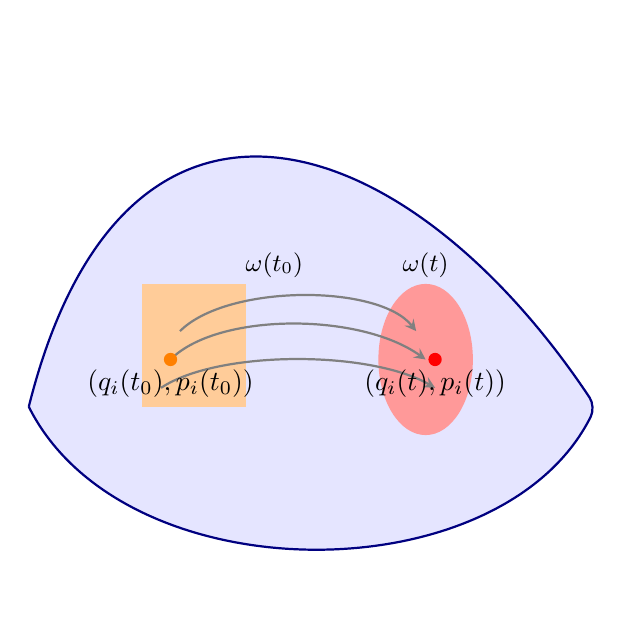
\begin{tikzpicture}[scale=1.2, >=stealth]

\fill[blue!10,rounded corners] (0,0) .. controls (1,4) and (4,3) .. (6 ,0)
                               .. controls (5,-2) and (1,-2) .. (0,0);
\draw[blue!50!black,thick,rounded corners] (0,0) .. controls (1,4) and (4,3) .. (6,0)
                                          .. controls (5,-2) and (1,-2) .. (0,0);

\fill[orange!40] (1.2,0.0) rectangle (2.3,1.3);
\node at (2.6,1.5) {\small \(\omega(t_0)\)};

\fill[red!40] (4.2,0.5) ellipse (0.5 and 0.8);
\node at (4.2,1.5) {\small \(\omega(t)\)};

\draw[->,thick,gray] (1.5,0.5) .. controls (2.0,1.0) and (3.5,1.0) .. (4.2,0.5);
\draw[->,thick,gray] (1.4,0.2) .. controls (2.0,0.6) and (3.6,0.6) .. (4.3,0.2);
\draw[->,thick,gray] (1.6,0.8) .. controls (2.1,1.3) and (3.7,1.3) .. (4.1,0.8);

\fill[orange] (1.5,0.5) circle (2pt) node[black,below] {$(q_i(t_0), p_i(t_0))$};
\fill[red] (4.3,0.5) circle (2pt) node[black,below] {$(q_i(t), p_i(t))$};
\end{tikzpicture}
\end{minipage}
\hfill
\begin{minipage}{0.48\textwidth}
    Initial condition \((q_i(t_0), p_i(t_0))\) evolves to \((q_i(t), p_i(t))\) under Hamiltonian flow. The volume of any region \(\omega(t_0)\) in phase space is preserved over time, i.e., \(\text{Vol}(\omega(t_0)) = \text{Vol}(\omega(t))\). Consequently, the density of states in phase space remains constant along the trajectories, which implies the conservation of the total number of states.
\end{minipage}
\end{figure}

\section{The Concept of State and Microstates}

Hamilton's equations are deterministic: once the initial conditions \(q_i(t_0), p_i(t_0)\) are specified, the system of first-order differential equations admits a unique solution \( (q_i(t), p_i(t)) \) for all times, provided the Hamiltonian is sufficiently smooth. Thus, the evolution in phase space is uniquely determined and reversible, as the flow defines a one-to-one mapping between initial and final states. Each such trajectory corresponds to a \textbf{microstate} of the system, fully characterizing its dynamical evolution.

However, in many practical situations, we are interested in systems where initial conditions are not precisely known, or where many microstates correspond to the same macroscopic description. This leads to the idea of a \textbf{macrostate}, characterized by thermodynamic variables like energy, volume, and particle number.

To study such systems, we introduce the concept of an \textbf{ensemble}: a large collection of copies of the system, all with the same macrostate but different microstates.

\subsection*{Probability Distributions in Phase Space}

For a large ensemble, we can define a probability density function \( p(q_i, p_i; t) \) on the phase space \( M \), such that:
\[
p(q_i, p_i; t) \geq 0, \quad \int_M p(q_i, p_i; t) \prod_i dq_i dp_i = 1.
\]

The probability of finding the system in a region \( \mathcal{U} \subset M^N \) is given by:
\[
\int_{\mathcal{U}} p(q_i, p_i; t) \prod_i dq_i dp_i.
\]

To make the measure dimensionless, we often use:
\[
d\Omega = \prod_i \frac{dq_i dp_i}{h},
\]
where \( h \) is a constant with units of action (e.g., Planck's constant).

\subsection*{Time Evolution and Stationarity}

The probability density evolves according to:
\[
\frac{dp}{dt} = \frac{\partial p}{\partial t} + \{p, H\} = 0.
\]

A system is \textbf{stationary} if \( \frac{\partial p}{\partial t} = 0 \), which is a necessary condition for thermodynamic equilibrium. In that case, \( \{p, H\} = 0 \), which holds if:
\begin{itemize}
    \item \( p = \text{constant} \) (microcanonical ensemble),
    \item \( p = p(H) \) (canonical or grand canonical ensemble).
\end{itemize}

The ensemble average of an observable \( f \) is defined as:
\[
\langle f \rangle = \int_M p(q_i, p_i) f(q_i, p_i) \prod_i dq_i dp_i,
\]
and its standard deviation is:
\[
(\Delta f)^2 = \langle f^2 \rangle - \langle f \rangle^2.
\]

\subsection*{Time-Independent Hamiltonians and Density of States}

When the Hamiltonian is time-independent, energy is conserved, and the system evolves on a constant-energy hypersurface in phase space.

The volume of phase space with energy between 0 and \( E \) is:
\[
\Sigma(E) = \int_{0 \leq H \leq E} \prod_i dq_i dp_i.
\]

The density of states is defined as:
\[
\omega(E) = \int_M \prod_i dq_i dp_i \, \delta(H(q_i, p_i) - E) = \frac{\partial \Sigma}{\partial E}.
\]

\section{Ergodicity}

The microcanonical average of an observable \( f \) on the energy surface \( S_E \) is:
\[
\langle f \rangle_E = \frac{1}{\omega(E)} \int_{S_E} f \, dS_E.
\]

The time average is:
\[
\langle f \rangle_\infty = \lim_{T \to \infty} \frac{1}{T} \int_{t_0}^{t_0+T} f(q_i(t), p_i(t)) \, dt.
\]

A system is \textbf{ergodic} if, for almost all initial conditions, the time average equals the microcanonical average:
\[
\langle f \rangle_\infty = \langle f \rangle_E.
\]

In what follows, we will assume ergodicity, which justifies the use of ensemble averages to describe thermodynamic equilibrium.